\documentclass[a4paper,11pt]{article}
\usepackage{a4wide}
\usepackage{fullpage}
\usepackage[utf8x]{inputenc}

\usepackage[light,math]{anttor}
\usepackage[T1]{fontenc}

%\usepackage[slovene]{babel}
%\selectlanguage{slovene}
\usepackage[toc,page]{appendix}
\usepackage[pdftex]{graphicx} 
\usepackage{amsfonts}
\usepackage{amsmath}
\usepackage{setspace}
\usepackage{color}
\definecolor{light-gray}{gray}{0.95}
\usepackage{listings} 
\usepackage{hyperref}
\renewcommand{\baselinestretch}{1.2} 
\renewcommand{\appendixpagename}{Priloge}

\lstset{ 
language=Matlab,
basicstyle=\footnotesize,
basicstyle=\ttfamily\footnotesize\setstretch{1},
backgroundcolor=\color{light-gray},
}

\usepackage{algorithm}
\usepackage[noend]{algpseudocode}


\title{Analysis of electrocardiographic (ECG) signals \\
with moving average based filtering for QRS detection}
\author{Sara Bizjak}
\date{\today}

\begin{document}

\maketitle

\section{Abstract}

\ \ This paper represents results of QRS detection algorithem summarized from the article \cite{bib:glavni} and tested on MIT/BIH Arrhythmia Database (source \cite{bib:net}).
The algorithm follows mentioned article entirely and has been tested with setting different parameters.
With chosen parameteres, the algorithm correctly detected over $99.2 \%$ of the QRS samples.

\section{Introduction}

\ \ QRS detection is a base for many automated cardiac signal analysis algorithms.
From many researches a lot of algorithms to detect QRS complex from the ECG (\textit{electrocardiogram}) have been developed.
While recording the ECG a lot of noise can be caught. Therefore, a reliable QRS detection algorithm is required to perform the ECG analysis.
In this paper, a simple and reliable (moving average-based real-time) QRS detection algorithm is presented and evaluated.

\section{Methodology}

\ \ Following the article, presented algorithm has three stages: a moving average-based linear \textit{high-pass filter} (HPF), a nonlinear \textit{low-pass filter} (LPF) and a decision-making stage.

\begin{figure}[ht!]
    \centering
    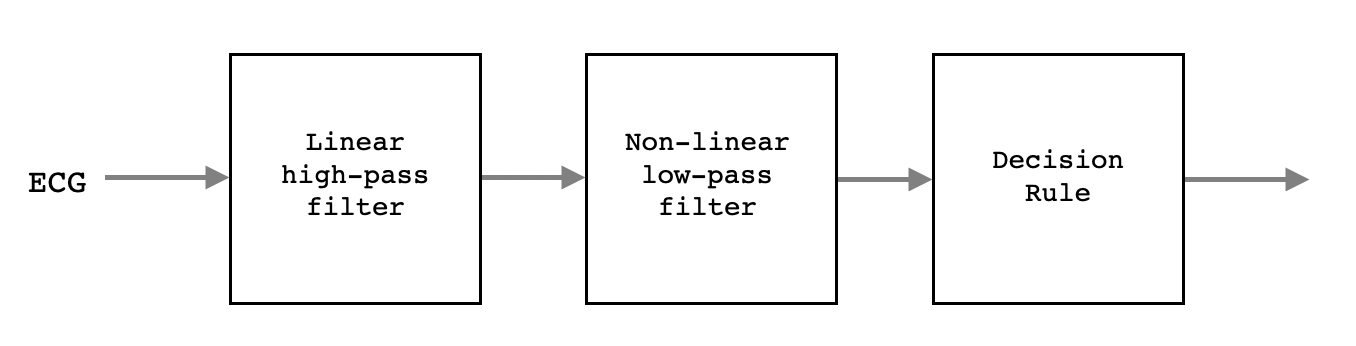
\includegraphics[width=130mm]{diagram.png}
    \caption{A diagram of the QRS detection system, summarized from article \cite{bib:glavni}.}
\end{figure}

\begin{figure}[ht!]
    \centering
    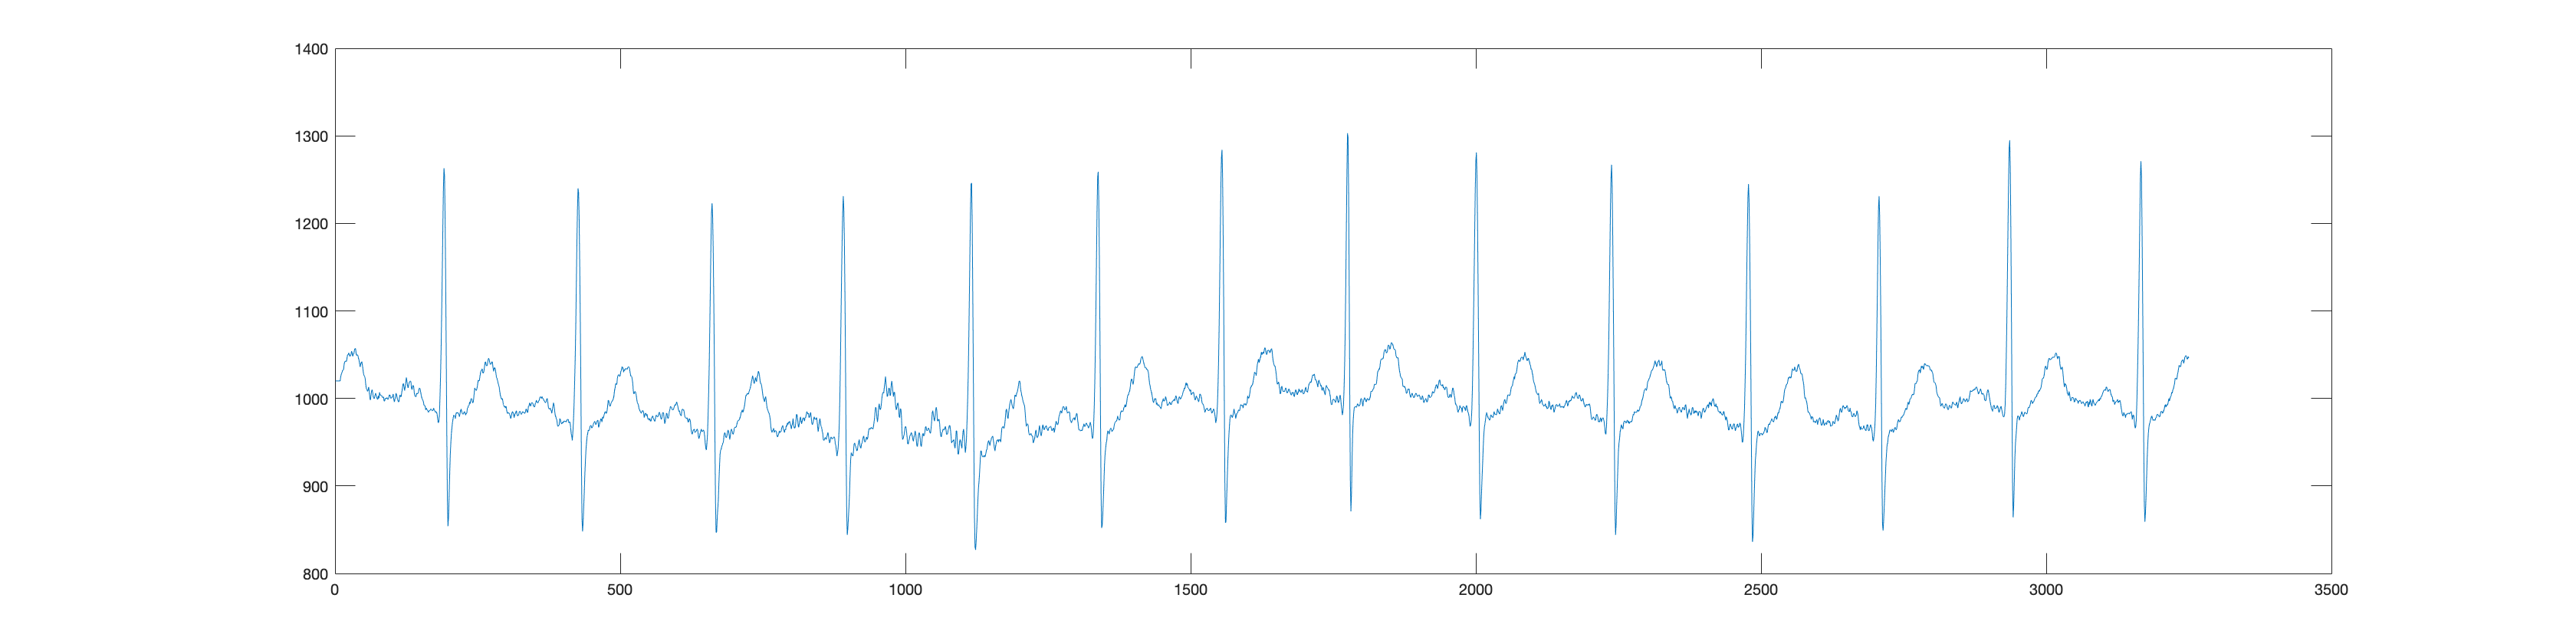
\includegraphics[width=160mm]{orig.png}
    \caption{Example of an ECG signal.}
\end{figure}

\newpage
\noindent
\ \ Firstly, the ECG recording is processed by the linear HPF in order to emphasize the QRS complex as well as to suppress the undesired waves of the ECG.

\begin{figure}[ht!]
    \centering
    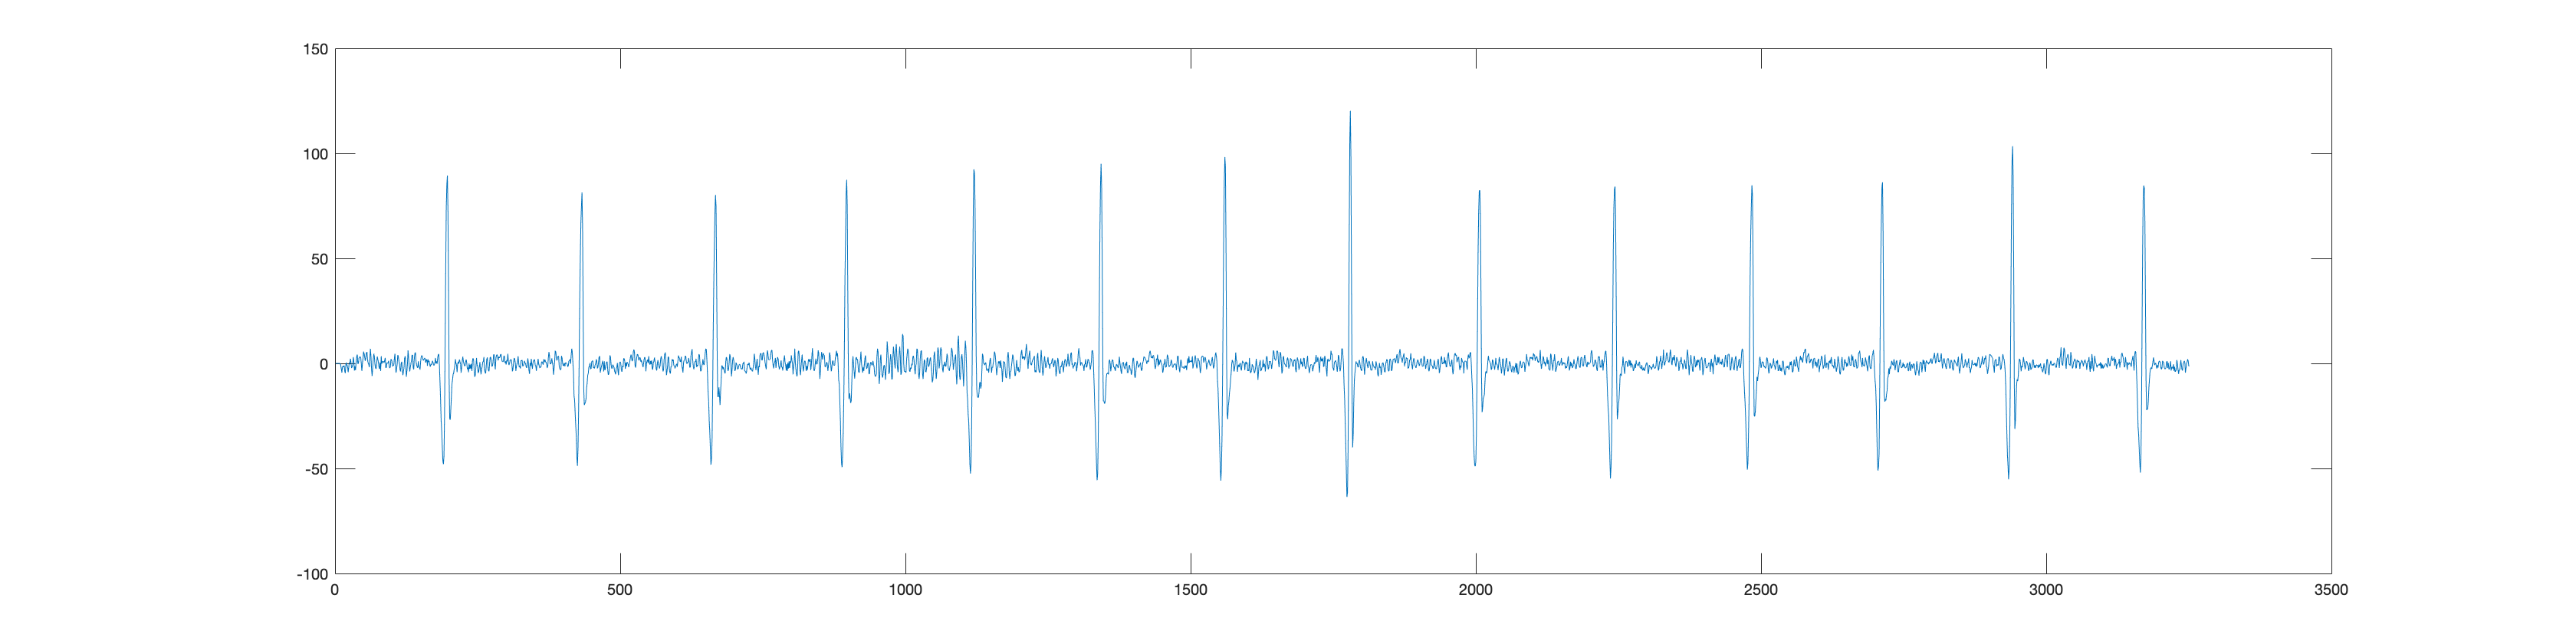
\includegraphics[width=160mm]{2.png}
    \caption{Example of filtered signal after first stage.}
\end{figure}
\noindent
\ \ Secondly, the linear HPF output is then processed by the non-linear LPF. 
LPF performs a non-linear amplification and full-wave rectification. 
LPF slides through signal with determined window size and sum squared points inside the current window. 
Since we square the points, all the negative values are lost and the signal is amplified.

\begin{figure}[ht!]
    \centering
    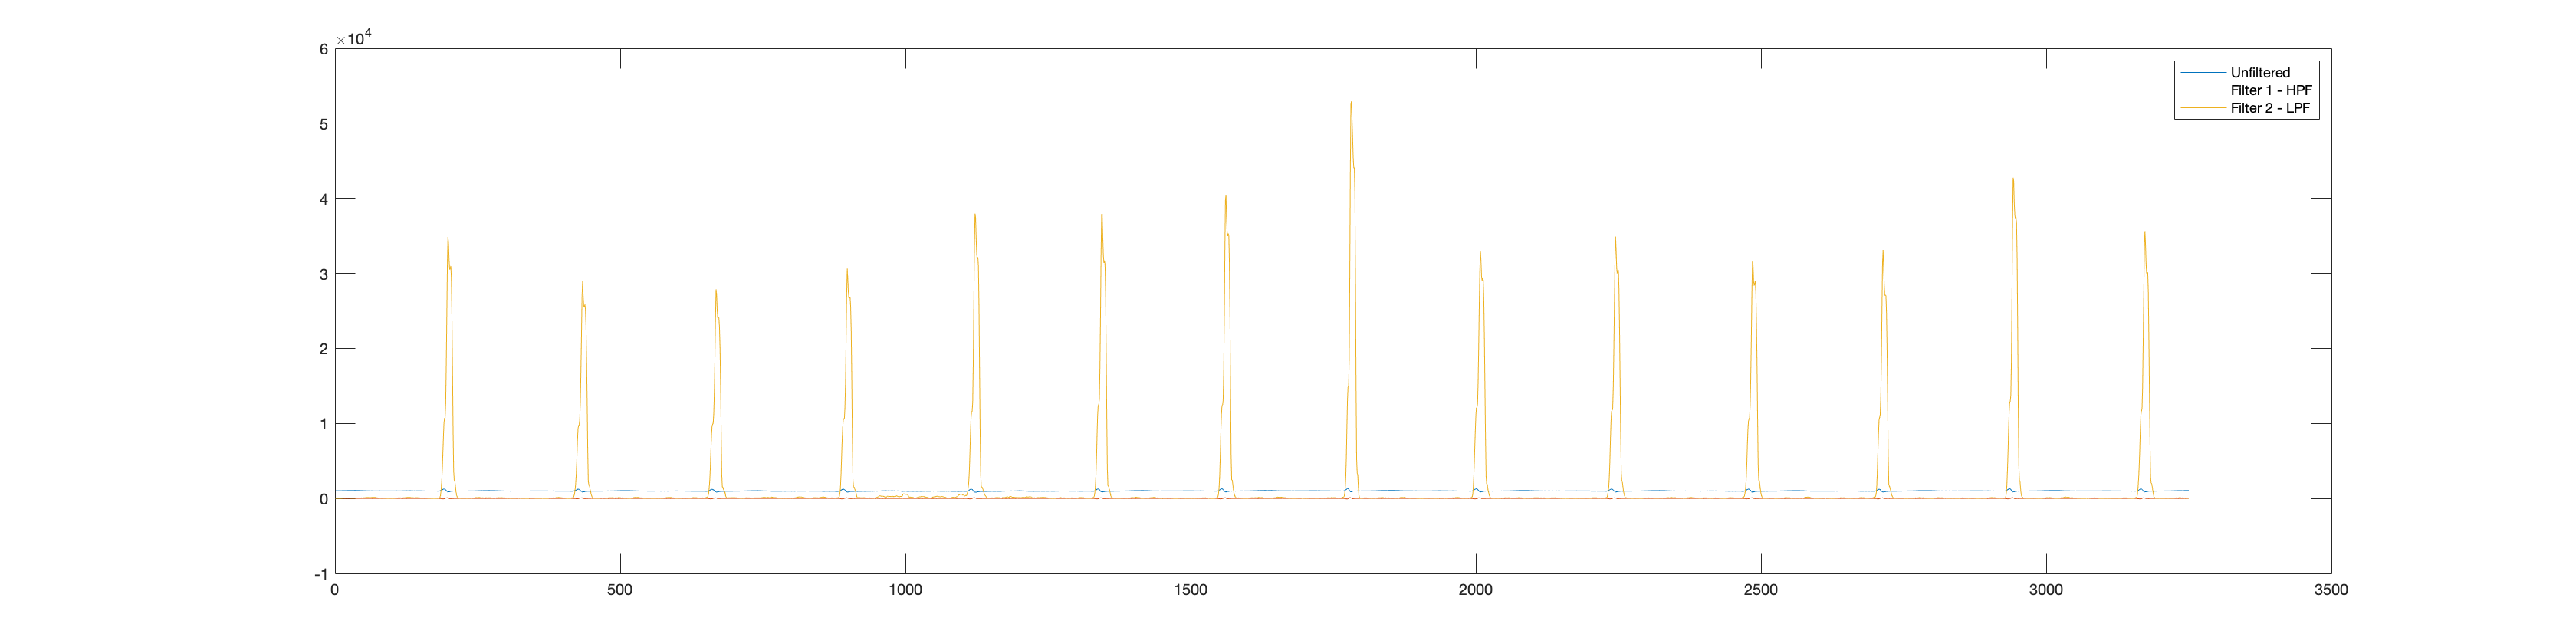
\includegraphics[width=160mm]{3.png}
    \caption{Example of filtered signal after second stage.}
\end{figure}
\noindent
\ \ Lastly, an adaptive threshold is applied and decision rule is completed, as well as the QRS detection.
Threshold is updated by the formula
$$ th = \alpha \times \gamma \times peak + (1 - \alpha) \times th $$
where $peak$ is the local maximum detected in the current waveform, $\alpha$ is the forgetting factor and $\gamma$ is a weighting factor. A QRS complex is detected if and only if the $peak$ level of the current signal exceeds the threshold. In that case, the threshold is updated. 

\section{Results}

\ \ The algorithm was tested against the 48 examples of MIT/BIH Arrhythmia Database.
Results were evaluated with the sensitivity and positive productivity.
$$ \text{Sensitivity:} \ Se = \frac{TP}{TP + FN} , $$
which is the proportion of events which were detected and presents an estimate of the likelihood of detecting an event.
$$ \text{Positive predictivity:} \ +P = \frac{TP}{TP + FP} , $$
which is the proportion of detections which actually were events and presents an estimate of the likelihood that s detection is an event.
\\
While testing, a lot of different combinations of parameters (as proposed in the article) were set. 
Although setting the size of a window for peak searching had to be tought well. 
It is important that size is not set too large, since two heartbeats could be caught in one window and consequently only one would be detected. Furthermore, it should also not be set to small.
\\
In the following table are presented parameters with best performance according to $Se$ and $+P$.

\begin{table}[ht!]
    \centering
    \begin{tabular}{|l|l|l|}
    \hline
    $\alpha$ & $0.05$ & forgetting factor       \\ \hline
    $\gamma$ & $0.15$ & weighting factor        \\ \hline
    $M$      & 5      & moving average window   \\ \hline
    $I$      & 10     & window size (summation interval)      \\ \hline
    $step$   & 180    & window size for peak (threshold) searching \\ \hline
    \end{tabular}
\end{table}
\noindent
Average sensitivity for tested samples is $99.2142 \%$ and average positive predictivity is $88.7438 \%$.

\section{Conclusion}

\ \ According to the results, the presented moving averaging-based QRS detection algorithm has high rate of sensitivity and is achieving high QRS detection rate. 
Based on observing sensitivity and positive predistivity, two algorithm improvements can be proposed.
Since the average positive predictivity is for around $10 \%$ lower than average sensitivity, we can conclude that the algorithm detects $10 \%$ more signals than are actually present,
hence the threshold is probably set to low.
The error could be reduced by improving the decision-making stage.
The results can be even more improved with setting parameters and choosing the best parameter combination for each database (or for similar databases). It could cost us more time, but the results should improve.
\\
To conclude, the algorithm -- despite its simplicity and low time complexity -- yields satisfactory results.

%%%%%%%%%%%%%%%%%%%%%%%%%%%%%%%%%%%%%%%%%%%

\begin{thebibliography}{99}

    \bibitem{bib:glavni}
    SW.~Chen, \emph{A Moving Average based Filtering System with its Applicationa to Real-time QRS Detection}, Computers in Cardiology \textbf{30} (2003) 585--588.

    \bibitem{bib:net}
    GB.~Moody, RG.~Mark \emph{The impact of the MIT-BIH Arrhythmia Database}, IEEE Eng in Med and Biol 20(3):45-50 (May-June 2001), (PMID: 11446209).

    \bibitem{bib:fisio}
    Goldberger, A.~Amaral, L.~Glass, L.~Hausdorff, J.~Ivanov, P.~C.~Mark, Stanley, H. E. (2000). PhysioBank, PhysioToolkit, and PhysioNet: \emph{Components of a new research resource for complex physiologic signals}, Circulation [Online]. 101 (23), pp. e215–e220.

\end{thebibliography}

\end{document}